\documentclass{article}
\usepackage[utf8]{inputenc}
\usepackage{amsmath,amsfonts,amssymb,amsthm,mathtools}
\usepackage{parskip}
\usepackage{color}
\usepackage{booktabs}

\newtheorem{exercise}{Exercise}
\newtheorem{answer}{Answer}

\newcommand{\dd}[2][]{\frac{\partial #1}{\partial #2}}
\newcommand{\yh}{\hat{y}}

\newcommand{\bracket}[3]{\left#1 #3 \right#2}
\newcommand{\sqb}{\bracket{[}{]}}
\renewcommand{\b}{\bracket{(}{)}}
\newcommand{\abs}{\bracket{\lvert}{\rvert}}

\newcommand{\x}{\mathbf{x}}
\newcommand{\y}{\mathbf{y}}
\newcommand{\f}{\mathbf{f}}
\newcommand{\X}{\mathbf{X}}
\newcommand{\W}{\mathbf{W}}
\newcommand{\I}{\mathbf{I}}
\renewcommand{\P}{\operatorname{P}\b}

\newcommand{\w}{\mathbf{w}}
\newcommand{\wo}{\w^*}

\renewcommand{\L}{\mathcal{L}}
\newcommand{\E}{\operatorname{E}\sqb}
\newcommand{\Var}{\operatorname{Var}\sqb}

\newcommand{\logits}{\ell}
\newcommand{\vlogits}{\boldsymbol{\logits}}
\newcommand{\softmax}{\operatorname{softmax}\b}

\title{EMAT31530, Part 3: Linear classification}
\author{Laurence Aitchison}
\date{}

\begin{document}

\maketitle



\section{We can't do gradient descent on the classification error}

Doing regression by gradient descent is pretty straightforward, because all the distances between the real data, $y_i$ and targets, $\yh(\x_i)$ are continuous and differentiable (almost everywhere).
However, things become much harder when it comes to classification.
For instance:
\begin{center}
  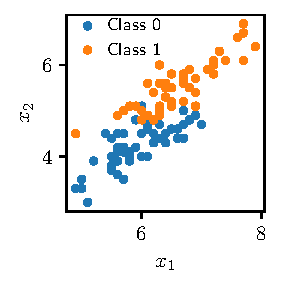
\includegraphics{clust_example.pdf}
\end{center}
Our goal is to learn a mapping from $\x \rightarrow y$ that looks like the mapping in the data.
For instance, we could use,
\begin{align}
  \yh_\w(\x) &= \Theta(\x \w)
\end{align}
where $\Theta(a)$ is the Heaviside step function, which returns $0$ when the input argument is negative ($a <0$), and returns $1$ otherwise.
\begin{center}
  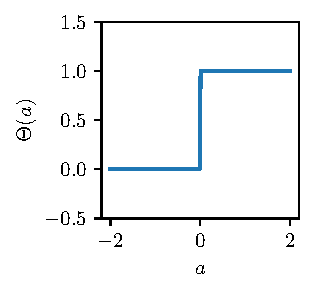
\includegraphics{heaviside.pdf}
\end{center}
As $\yh_\w(\x)$ returns $0$ or $1$, and is parameterised in terms of a weight-vector, $\w$, we can treat the output from $\yh_\w(\x)$ as a prediction of the class (class $0$ or class $1$). We can then optimize the weights in order to give better predictions.

Key problem: what loss function to use?
The obvious choice is classification error:
\begin{align}
  \label{eq:class_error}
  \L(\w) &= \text{number of wrong classifications}\\
  &= \sum_{i=1}^N \text{different}(y_i, \yh_\w(\x_i))
  \intertext{where,}
  \text{different}(y, \hat{y}) &= 
  \begin{cases} 
    0 &\text{if } y = \hat{y}\\
    1 &\text{otherwise}
  \end{cases}
\end{align}
The problem is that the number of wrong classifications is always an integer (0, 1, 2 etc.)
\begin{center}
  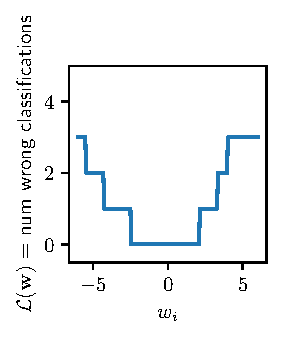
\includegraphics{non_diff_loss.pdf}
\end{center}
This function isn't continuous. In fact, the gradient is flat (almost) everywhere! So we can't do gradient descent!

Instead, we need an alternative loss, which is continuous and differentiable (almost everywhere).
How do we get such a loss?
We're going to set up classification as maximum-likelihood in a probabilistic model.  To introduce the basic idea, we first need to take a detour through maximum-likelihood for coin flipping...

\section{Maximum likelihood for coin flipping}

%That's all fine at a very high-level.
%But to ground everything, we need to start by working with a concrete distribution, $\P{x| \theta}$.
%Perhaps the simplest concrete distribution arises from tossing a biased coin.
%We're therefore going to use maximum likelihood to fit the probability, $p$.
%Once we have $p$, we can also sample new coin tosses that look like those in the data.

When tossing a biased coin, our random variable, $x$, can take on values of $1$ or $0$.
In coin flipping, $x=1$ corresponds to heads and $x=0$ corresponds to tails.
In classification (which we'll get on to), $x=1$ corresponds to class 1, while $x=0$ corresponds to class $0$ (logically enough).
Because this is a biased coin, there is a parameter, $p$, which controls the probability of heads vs tails (or $x=1$ vs $x=0$).
Specifically, the probability is,
\begin{subequations}
\begin{align}
  \label{eq:bern}
  \P{x=1| p} &= p\\
  \P{x=0| p} &= (1-p).
\end{align}
\end{subequations}
The probability of heads \textit{or} tails adds to $1$,
\begin{align}
  1 = \P{x=1| p} + \P{x=0| p} &= p + (1-p).
\end{align}
For the maths, it'll be super-useful to have a form for the probability which takes $x$ as an input (rather than just having two different forms for $x=1$ and $x=0$, as in Eq.~\ref{eq:bern}).
We can write this as,
\begin{align}
  \label{eq:coin}
  \P{x| p} &= p^x (1-p)^{1-x}
  \intertext{Note that there isn't really a ``derivation'' for this.  It just happens to be a general form that gives the right answer when we substitute $x=1$ and $x=0$,}
  \P{x=1| p} &= p^1 (1-p)^0 = p \times 1 = p,\\
  \P{x=0| p} &= p^0 (1-p)^1 = 1 \times (1-p) = (1-p).
\end{align}

Anyway: lets get back to our maximum likelihood problem.  We have a dataset of tosses from a biased coin, $x_1,\dotsc,x_N$.
Our goal is to estimate the probability, $p$, that generated these coin tosses.
To do that, we find the $p$ that makes the observed data most probable. 
\begin{align}
  \L(p) &= \log \P{x_1,\dotsc,x_N| p}
\end{align}
Specifically, we maximize the maximize the \textit{log} probability, for the reasons in the Prerequisites part:
\begin{itemize}
  \item The logarithm is a monotonically increasing function, so the maximum of the probability as a function of the parameter, $p$ is the same place as the maximum of the log-probability as a function of $p$.      
  \item Logarithms turn products into sums, and its much easier to differentiate sums than products.
  \item Raw probabilities can be very large or very small once we take products over a large number of datapoints.  That can cause numerical issues (i.e. over/underflow).  
\end{itemize}
We assume that coin tosses are independent, so $\P{x_1,\dotsc,x_N| p} =\prod_{i=1}^N \P{x_i| p}$, and 
\begin{align}
  \L(p) &= \log \prod_{i=1}^N \P{x_i| p} \\
  \intertext{The log turns the product into a sum,}
  \L(p) &= \sum_{i=1}^N \log \P{x_i| p}\\
  \intertext{Substituting the log-probability for tossing a biased coin (Eq.~\ref{eq:coin}),}
  \L(p) &= \sum_{i=1}^N \log \b{p^{x_i} (1-p)^{1-x_i}}\\
  \intertext{The log again turns the product into a sum,}
  \L(p) &= \sum_{i=1}^N \b{\log\b{p^{x_i}} + \log\b{(1-p)^{1-x_i}}}
  \intertext{And the log turns powers into products,}
  \label{eq:coin_flip_prob}
  \L(p) &= \sum_{i=1}^N \b{x_i\log p + (1-x_i) \log(1-p)}
  \intertext{Applying the sum to each term separately, and noting that $p$ is independent of $i$,}
  \L(p) &= \b{\sum_{i=1}^N x_i} \log p + \b{\sum_{i=1}^N (1-x_i)}\log(1-p)
  \intertext{And finally, separating out the two terms in the second sum,}
  \label{eq:coin_flip_ll}
  \L(p) &= \underbrace{\b{\sum_{i=1}^N x_i}}_{\text{a constant number}} \log p + \underbrace{\b{N - \sum_{i=1}^N x_i}}_{\text{another constant number}}\log(1-p)
  \intertext{So we can treat this as,}
  \L(p) &= a \log p + b \log(1-p)
\end{align}
where,
\begin{align}
  a &= \sum_{i=1}^N x_i&
  b &= N - \sum_{i=1}^N x_i
\end{align}
Notice that we've extracted the sums over data into constant multipliers, $a$ and $b$.
This has simplified the loss, $\L(p)$, dramatically.
So finding the maximum-likelihood value for $p$ is now a calculus problem!

Moreover, notice that despite the data, $x_i$, being discrete, the objective is a continuous and differentiable function of the parameter, $p$. 
As such, we can find the most likely probability, $p^*$, by doing gradient descent!
If we did that, we'd end up with the sensible answer (see Exercises),
\begin{align}
  p^* &= \tfrac{1}{N} \sum_{i=1}^N x_i.
\end{align}


\section{A smooth, maximum-likelihood objective for binary classification}
\label{sec:binary_obj}
In the previous section, we saw that we can get a continuous, differentiable loss for discrete data by setting the problem up as maximum-likelihood.
So how do we apply the same idea to get a differentiable loss for binary classification?
The basic idea is that we first use a bunch of weights to get ``logits'',
\begin{align}
  \logits = f_\w(\x_i) &= \x_i \w
\end{align}
The problem is that the logits could be from $-\infty$ to $\infty$, while we want a probability, between $0$ and $1$.
To solve this problem, we transform the logits by applying a function, the ``logistic sigmoid'' (or sigmoid for short), denoted $p = \sigma(\logits)$ from a logits in $-\infty$ to $\infty$, to a probability from $0$ to $1$.
Specifically, the probability is,
\begin{align}
  \label{eq:sigmoid_prob}
  p_\w(\x) &= \sigma(\logits = f_\w(\x_i))
\end{align}
The key question is then how do we define the sigmoid function, $\sigma$, to solve these problems?
Answer: the sigmoid function!
\begin{align}
  \sigma(\logits) &= \frac{1}{1+e^{-\logits}}
\end{align}
The sigmoid function takes any $\logits$ (from $-\infty$ to $\infty$) and returns a number from $0$ to $1$:
\begin{center}
  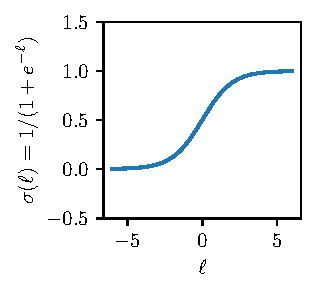
\includegraphics{sigmoid.pdf}
\end{center}
As such, the sigmoid does indeed give a valid probability (i.e.\ a number between $0$ and $1$).

\section{A smooth, maximum-likelihood objective for multi-class classification}
\label{sec:multi_obj}
In the last section, we were looking at classification problems where there's two possible classes.
But almost always, there's multiple classes.
For instance, we might want to classify handwritten digits as 0--9, in which case, there's ten classes.
\begin{center}
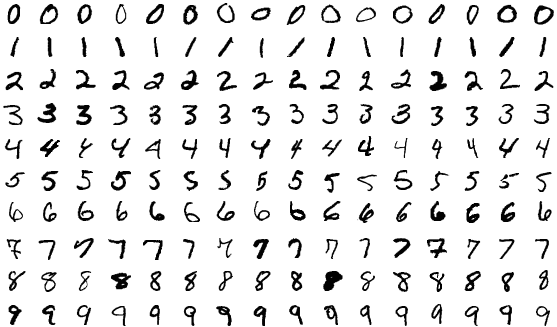
\includegraphics[width=0.7\textwidth]{mnist}
\end{center}
Again, to train a model for multi-class classification, we need an objective.
Classification error (Eq.~\ref{eq:class_error}) also makes sense in the multi-class setting, but again, can't be used as an objective as it is non-differentiable.
As in the binary classification setting, we need an objective that is a continuous, differentiable function of the parameters (weights).
To get such an objective, we're again going to consider a probability distribution over classes.
In multi-class classification, the probability distribution is over the integers $0$--$9$ (or in general, over the integers $0$--$C$, where $C$ is the number of classes), instead of just over $\{0, 1\}$.

The first problem is that previously, we just had one scalar logits for each datapoint, $\logits = f_\w(\x_i) = \x_i \w$. 
It is not at all clear how to turn that scalar into a probability distribution over multiple classes.
As such, in multi-class classification, we use a whole \textit{vector} of logits, $\vlogits$, for each datapoint.
This vector has length $C$, so there's one logits for each class,
\begin{align}
  \underbrace{\vlogits}_{1 \times C} = \f_{\W}(\x) = \underbrace{\x}_{1 \times D} \underbrace{\W}_{D \times C}.
\end{align}
Note that we get a vector of logits by changing the usual $D \times 1$ weight vector, $\w$, with a $D\times C$ weight matrix, $\W$.

Again, we have the problem of how to set the probability for each class, given that the individual logits values can be anywhere from $-\infty$ to $\infty$.
\begin{align}
  p_c(\x) &= \softmax{\vlogits = \f_{\W}(\x)} = \frac{e^{\logits_c}}{\sum_{c'} e^{\logits_{c'}}}
\end{align}
where $c$ is the class label.
Remember that the probabilities must all be bigger than $0$ and sum to $1$.
It is straightforward to check that the resulting probabilities sum to $1$,
\begin{align}
  \sum_{c} p_c(\x) &= \frac{\sum_c e^{\logits_c}}{\sum_{c'} e^{\logits_{c'}}} = 1
\end{align}
as the numerator and denominator are the same.

\section{Gradient descent for binary classification}
Now, we have discussed the loss function for binary and multiclass classification, we need to think about how to actually use this objective to optimize the weights.
We'll focus on the binary setting (to keep things slightly simpler) and use gradient descent.
But first-things-first, it turns out to be useful to rearrange the objective itself into a simpler form.
Remember that the objective is the log-probability of class-labels under our model,
\begin{align}
  \L(\w) &= \log \P{y_1,\dotsc,y_N| \w, \x_1,\dotsc,\x_N}\\
  \intertext{The class-labels for different inputs are independent,}
  \L(\w) &= \sum_{i=1}^N \log \P{y_i| \w, \x_i}\\
  \intertext{Using the coin-flipping probability from Eq.~\eqref{eq:coin}}
  \L(\w) &= \sum_{i=1}^N \log (p_{\w}(\x_i)^{y_i} (1-p_{\w}(\x_i))^{1-y_i})\\
  \intertext{The log turns products into sums,}
  \L(\w) &= \sum_{i=1}^N \sqb{\log (p_{\w}(\x_i)^{y_i}) + \log((1-p_{\w}(\x_i))^{1-y_i})}.\\
  \intertext{Next, the log turns powers into products, (mirroring the coin flipping result in Eq.~\ref{eq:coin_flip_prob})}
  \L(\w) &= \sum_{i=1}^N \sqb{y_i\log (p_{\w}(\x_i)) + (1-y_i)\log((1-p_{\w}(\x_i)))}.\\
  \intertext{Substituting the value of $p_{\w}(\x)$ (Eq.~\ref{eq:sigmoid_prob}), (keeping the sigmoid in the first term, but using the explicit form for the sigmoid in the second term),}
  \L(\w) &= \sum_{i=1}^N \sqb{y_i\log \sigma(\w^T \x) + (1-y_i)\log\b{1 - \frac{1}{1+e^{-\w^T \x}}}}
  \intertext{Using, $1 = (1+e^{-\w \x_i^T}) /(1+e^{-\w \x_i^T})$,}
  \L(\w) &= \sum_{i=1}^N \sqb{y_i\log \sigma(\w^T \x_i) + (1-y_i)\log\b{\frac{1+e^{-\w \x_i^T}}{1+e^{-\w \x_i^T}} - \frac{1}{1+e^{-\w^T \x}}}},\\
  \L(\w) &= \sum_{i=1}^N \sqb{y_i\log \sigma(\w^T \x_i) + (1-y_i)\log\frac{1 +e^{-\w^T \x_i} - 1}{1+e^{-\w^T \x_i}}},\\
  \L(\w) &= \sum_{i=1}^N \sqb{y_i\log \sigma(\w^T \x_i) + (1-y_i)\log\frac{e^{-\w^T \x_i}}{1+e^{-\w^T \x_i}}}.
  \intertext{Multiplying the numerator and denominator by $e^{\w^T \x}$,}
  \L(\w) &= \sum_{i=1}^N \sqb{y_i\log \sigma(\w^T \x_i) + (1-y_i)\log\frac{(e^{-\w^T \x_i}) e^{\w^T \x_i}}{(1+e^{-\w^T \x_i}) e^{\w^T \x_i}}},\\
  \L(\w) &= \sum_{i=1}^N \sqb{y_i\log \sigma(\w^T \x_i) + (1-y_i)\log\frac{1}{1 + e^{\w^T \x_i}}}
  \intertext{Finally, notice that the final term is another sigmoid,}
  \L(\w) &= \sum_{i=1}^N \sqb{y_i\log \sigma(\w^T \x_i) + (1-y_i)\log \sigma(-\w^T \x_i)}
\end{align}

Now, we want to differentiate this objective wrt a weight.
This is a bigger, more complicated and scarier function than any we've seen before.
But things are going to be okay if we write out a stepwise process for computing the function, and apply the chain rule everywhere!
Specifically, we're going to compute the chain-rule using the following sequence of computations.
We're first going to compute the product of features and weights,
\begin{align}
  a^i &= \sum_\lambda w_\lambda X_{\lambda i}\\
  \intertext{Then we're going to apply the sigmoid,}
  s^i_0 &= \sigma(-a^i) &
  s^i_1 &= \sigma(a^i),\\
  \intertext{Then we're going to apply the log,}
  l^i_0 &= \log s^i_0 & 
  l^i_1 &= \log s^i_1,
  \intertext{Then we're going to compute the objective,}
  \L(\w) &= \sum_{i=1}^N \sqb{y_i l^i_1 + (1-y_i) l^i_0}.
\end{align}
The gradient is therefore,
\begin{align}
  \dd[\L(\w)]{w_\nu} &= \sum_{i=1}^N \sqb{y_i \dd[l^i_1]{w_\nu} + (1-y_i) \dd[l^i_0]{w_\nu}}.
  \intertext{Applying the chain rule,}
  \dd[\L(\w)]{w_\nu} &= \sum_{i=1}^N \sqb{y_i \dd[l^i_1]{s^i_1} \dd[s^i_1]{a^i_1} \dd[a^i]{w_\nu} + (1-y_i) \dd[l^i_0]{s^i_0} \dd[s^i_0]{a^i} \dd[a^i_0]{w_\nu}}.
\end{align}
Now, we need to compute the individual derivatives in the chain rule.
To start, we look at the linear combination of weights and features,
\begin{align}
  \dd[a^i]{w_\nu} &= \dd{w_\nu}\sqb{\sum_\lambda w_\lambda X_{\lambda i}} = \sum_\lambda \delta_{\nu \lambda} X_{\lambda i} = X_{\nu i}\\
  \intertext{(see the last exercise of ``Mathematical Prerequisites'' for details).  For the sigmoid (you're going to work out the form for this derivative in the exercises)}
  \dd[s^i_0]{a^i} &= \dd[\sigma(-a^i_0)]{a^i_0} = -\sigma(a^i) \sigma(-a^i)\\
  \dd[s^i_1]{a^i} &= \dd[\sigma(a^i_1)]{a^i_1} = \sigma(a^i) \sigma(-a^i)\\
  \intertext{And finally the log,}
  \dd[l^i_0]{s^i_0} &= \dd[\log s^i_0]{s^i_0} = \frac{1}{s^i_0} = \frac{1}{\sigma(-a^i)}\\
  \dd[l^i_1]{s^i_1} &= \dd[\log s^i_1]{s^i_1} = \frac{1}{s^i_0} = \frac{1}{\sigma(a^i)}
\end{align}
Putting everything back together, we get something reasonably simple,
\begin{align}
  \dd[\L(\w)]{w_\nu} &= \sum_{i=1}^N \sqb{y_i \dd[l^i_1]{s^i_1} \dd[s^i_1]{a^i_1} \dd[a^i_1]{w_\nu} + (1-y_i) \dd[l^i_0]{s^i_0} \dd[s^i_0]{a^i_0} \dd[a^i]{w_\nu}}\\
  &= \sum_{i=1}^N X_{i \nu} \sqb{y_i \sigma(-a^i) - (1-y_i) \sigma(a^i)}
\end{align}
While we \textit{could} compute these derivatives, it was pretty darn tedious.
It would be great if we could get the computer to do it for us!
Next week, we're going to look at neural networks themselves, and see that PyTorch somehow magically computes the gradients for us.
The week after, we're going to see precisely \textit{how} PyTorch does this magic!


\section{Exercises}

\begin{exercise}
  Find the maximum-likelihood probability for a biased coin, given a dataset of $N$ tosses, $x_i$, with $x_i=0$ representing tails and $x_i=1$ representing heads.
  Start from the expression for the log-likelihood in Eq.~\ref{eq:coin_flip_ll}, and solve for the value of $p$ at which the gradient of the log-likelihood is zero.
\end{exercise}

\begin{exercise}
  Show that the gradient of a sigmoid is
  \begin{align}
    \dd[\sigma(a)]{a} = \sigma(a) \sigma(-a)
  \end{align}
\end{exercise}

\section{Answers}


\begin{answer}
Now, we find the maximum likelihood value of $p$ by solving for where the gradient is zero,
\begin{align}
  0 &= \dd[\L(p)]{p} \\
  0 &= \b{\sum_{i=1}^N x_i} \dd[\log p]{p} + \b{N - \sum_{i=1}^N x_i} \dd[\log(1-p)]{p}
\end{align}
It is a standard result that,
\begin{align}
  \dd[\log p]{p} &= \frac{1}{p}.
  \intertext{But to compute the other derivative, we need to apply the chain rule.  Specifically, we use,}
  u &= (1-p)\\
  y &= \log(1-p) = \log u.
  \intertext{Thus,}
  \dd[y]{p} &= \dd[y]{u} \dd[u]{p}\\
   &= \dd[\log u]{u} \dd{p}[1-p]\\
   &= \frac{1}{u}\times(-1)\\
   &= - \frac{1}{1-p}
\end{align}
Substituting in the derivatives,
\begin{align}
  0 &= \b{\sum_{i=1}^N x_i}\frac{1}{p} - \b{N - \sum_{i=1}^N x_i} \frac{1}{1-p}
  \intertext{To get the $p$'s out of the denominators, we multiply both sides by $p (1-p)$,}
  0 &= \b{\sum_{i=1}^N x_i}\frac{p (1-p)}{p} - \b{N - \sum_{i=1}^N x_i} \frac{p (1-p)}{1-p}\\
  0 &= \b{\sum_{i=1}^N x_i}(1-p) - \b{N - \sum_{i=1}^N x_i} p
  \intertext{Now, we separate out all the terms,}
  0 &= \b{\sum_{i=1}^N x_i} - \b{\sum_{i=1}^N x_i}p - N p + \b{\sum_{i=1}^N x_i} p.
  \intertext{And cancel the second and fourth term,}
  0 &= \b{\sum_{i=1}^N x_i} - N p.
  \intertext{Now, we add $N p$ to both sides,}
  Np &= \sum_{i=1}^N x_i
  \intertext{And divide both sides by $N$,}
  p &= \tfrac{1}{N} \sum_{i=1}^N x_i.
\end{align}
\end{answer}

\begin{answer}
  Find the gradient of a sigmoid,
  \begin{align}
    \dd[\sigma(a)]{a} &= \dd{a} \frac{1}{1+e^{-a}}
    \intertext{Apply the chain rule, with $u=1+e^{-a}$,}
    \sigma(a) &= u^{-1}
    \dd[\sigma(a)]{a} &= \dd[u^{-1}]{u} \dd[u]{a}
    \intertext{The individual derivatives are,}
    \dd[u^{-1}]{u} &= -u^{-2}\\
    \dd[u]{a} &= \dd{a}\sqb{1+e^{-a}} = - e^{-a}
    \intertext{Putting everything back together,}
    \dd[\sigma(a)]{a} &= \dd[u^{-1}]{u} \dd[u]{a} = \frac{e^{-a}}{u^2} = \frac{e^{-a}}{(1+e^{-a})^2}
    \intertext{Split up the denominator,}
    \dd[\sigma(a)]{a} &= \frac{1}{(1+e^{-a})} \frac{e^{-a}}{(1+e^{-a})}\\
    \intertext{The first term is a sigmoid, and in the second term, we divide the numerator and denominator by $e^{-a}$,}
    \dd[\sigma(a)]{a} &= \sigma(a) \frac{1}{(1+e^a)}\\
    \intertext{So the second term is also a sigmoid, just with the argument negated,}
    \dd[\sigma(a)]{a} &= \sigma(a) \sigma(-a).
  \end{align}
\end{answer}

\end{document}

